\chapter{Proposal} \label{proposal}

The main purpose of this proposal is the definition of a \textsc{DSL} that allows the specification of all different kinds of sentences, and afterwards, the possibility of testing given sentences as input and check if they are written accordingly to the rules previously specified. One obstacle that was encountered was how to extract the lexical part of the sentence, and in what way would each component be classified. In fact, this task is quite subjective, as different components may have various definitions in one context. % for example: (...). % Introduzir exemplo da professora!!!! 
Having known this, the decision was made that the student would beforehand identify the lexical part of the sentence.
% FALAR DO QUE VOU FAZER DE DIFERENTE (DICA DO LÁZARO!)

\section{System Architecture}
In order to specify all kinds of sentences/rules possible, the idea of creating a ``meta-language'' emerged. This ``meta-language'' is suppost to be the language in which the teacher would specify the rules for sentence construction. These rules would be written (in a single file) according to the following structure, that is divided into three main categories:

\begin{enumerate}
    \item \textbf{STRUCTURE} - this would be the block where the teacher would write how was the sentence suppost to be written, and what components would it have.
    
    \item \textbf{ERRORS} - list of conditions that the teacher would write in order to be analysed afterwards, for example, certain values for different attributes. If one of the conditions was matched, an error would appear.
    
    \item \textbf{INPUT} - this block corresponds to the ``parsing'' of the sentence (the lexical part) that the student wants to test. This would be written by the student and then automatically joined with the teachers information.
\end{enumerate}

This file would then be processed by an \textsc{ANTLR} processor that would work on the information that was written, and then generate a grammar (also specified in \textsc{ANTLR}). This grammar corresponds to the translation of the ``meta-language'' into \textsc{ANTLR} instructions. Afterwards, the generated grammar would be used to create a validator of sentences, where the student could write his sentence/sentences and obtain results. These results would be the validation of the given sentence/sentences and a tree for a better visualization of the input structure.

% Imagem da arquitetura do sistema.
\begin{figure}[h]
    \centering
    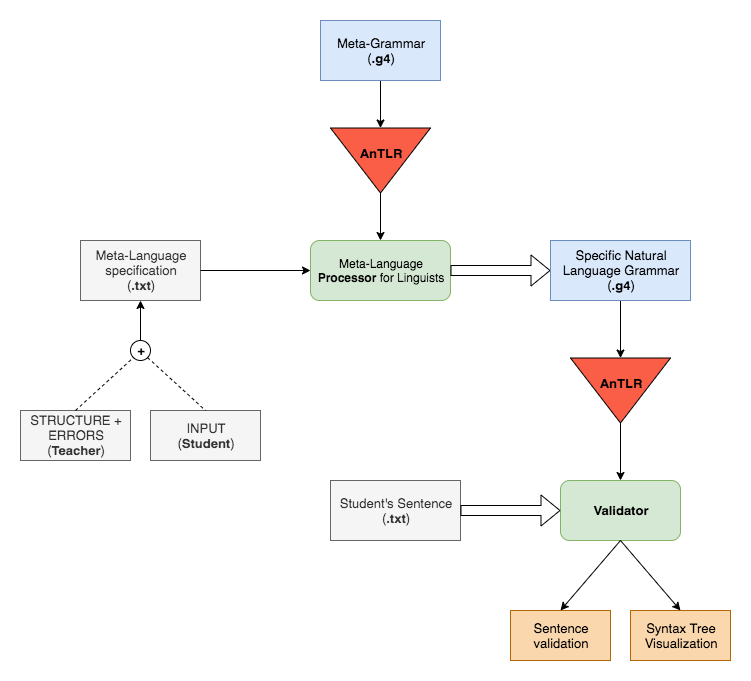
\includegraphics[width=12cm]{images/msc_system_architecture.png}
    \caption{System architecture.}
    \label{fig:system_architecture}
\end{figure}

\section{Meta-Language}
As it was stated in the beginning of this document, the main goal was to create a \textsc{DSL} that was easy to learn and to rapidly understand and grasp. With this in mind, the structure mencioned before on the first section of this chapter was followed: Three main parts, where two of them would be constructed by the teacher, and the third one was intended to be written by the student and later concatenated in a single file.

\subsection{Domain Specific Meta-Grammar}
The main intention of this language is to preprocess the information written by the teacher + student and then generate a validator for a particular structure. With simplicity in mind, a first version of the \textsc{DSL} was created, and it will be explained next.

\begin{figure}[h]
    \centering
    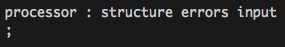
\includegraphics[width=7cm]{images/META_processor.png}
    \caption{DSL processor production.}
    \label{fig:dsl_processor_production}
\end{figure}

Firstly, the teacher specification will be discussed - meaning the \textbf{structure} and \textbf{errors} blocks.
The \textbf{structure} block is divided into \textbf{parts}, or main parts. These main parts correspond to the main components of the sentence. Each of these parts have an \textbf{element} within, containing the information about a certain component.

\begin{figure}[h]
    \centering
    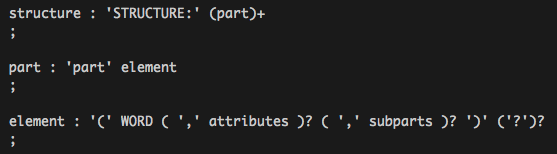
\includegraphics[width=10cm]{images/META_structure.png}
    \caption{DSL structure/part/element productions.}
    \label{fig:dsl_structure_production}
\end{figure}

The \textbf{element} is composed by the name of the component, a possible set of \textbf{attributes} and possible \textbf{subparts}.

\begin{figure}[h]
    \centering
    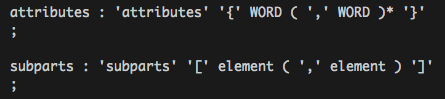
\includegraphics[width=8cm]{images/META_attributes_subparts.png}
    \caption{DSL attributes/subparts productions.}
    \label{fig:dsl_attributes_production}
\end{figure}

The \textbf{subparts} production intends to be the path for ``injecting'' more elements inside a single component. One component may be composed by several other components. As shown in the example above, the \textbf{subparts} production is a list of one or more elements.

Secondly, the teacher can define a list of restrictions to be applied to each attribute defined in the previous structure. These restrictions are logical conditions that must be obey for a sentence to be valid based on a specific structure.

\begin{figure}[h]
    \centering
    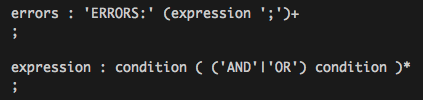
\includegraphics[width=8cm]{images/META_errors.png}
    \caption{DSL errors/expression productions.}
    \label{fig:dsl_errors_production}
\end{figure}

The \textbf{expression} production is a set of conditions that can be joined using the logical operators 'AND' and 'OR'. Each condition intends to access each attribute of any component and then assign it a value.

\begin{figure}[h]
    \centering
    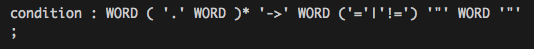
\includegraphics[width=10cm]{images/META_condition.png}
    \caption{DSL condition production.}
    \label{fig:dsl_condition_production}
\end{figure}

If, for instance, the teacher says that an attribute is equal to some value, then the student can not use said value with said attribute - this would result in an error.

Thirdly, and finally, the \textbf{input} block, which corresponds to the students section. This was treated has a different and separate \textsc{DSL}, as its main purpose was to identify the lexical parts of the sentence written by the student, allowing for a correct and non-subjective parsing of each word in the sentence. It is also important to notice that this first sketch is still \underline{verbose}, with only functionality in mind. By being treated as a separate \textsc{DSL}, it is accessible when it comes to changes, and simple to produce them.

\begin{figure}[h]
    \centering
    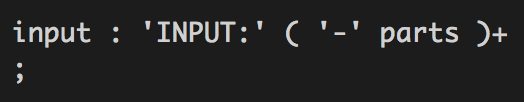
\includegraphics[width=7cm]{images/META_input.png}
    \caption{DSL input production.}
    \label{fig:dsl_input_production}
\end{figure}

The sketch starts within a section named \textbf{parts}, which corresponds to one sentence in particular. This production is composed by one or more blocks, where all the information is stored. Inside, the name of the components and their required attributes must be specified. It is also important to notice that a correct path must be specified by the student. If the student specifies a component that is not declared in the structure defined previously by the teacher, then an error should be thrown.

\begin{figure}[h]
    \centering
    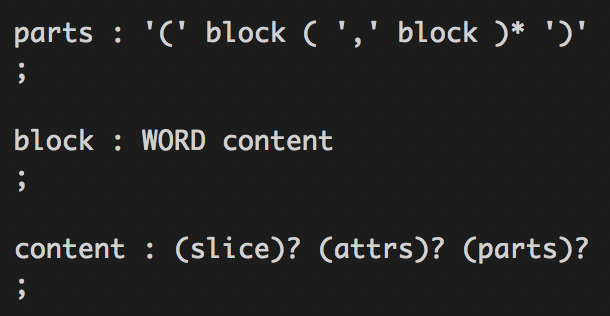
\includegraphics[width=8cm]{images/META_parts.png}
    \caption{DSL parts/component/content production.}
    \label{fig:dsl_parts_production}
\end{figure}

The student can specify the \textbf{slice} of the sentence that corresponds to the component that is being declared, and a set of attributes (\textbf{attrs}) that composes said component. Furthermore, it is possible to continue to define more \textbf{parts} within one part, just like the teacher's \textsc{DSL} \textbf{subparts}.

\begin{figure}[h]
    \centering
    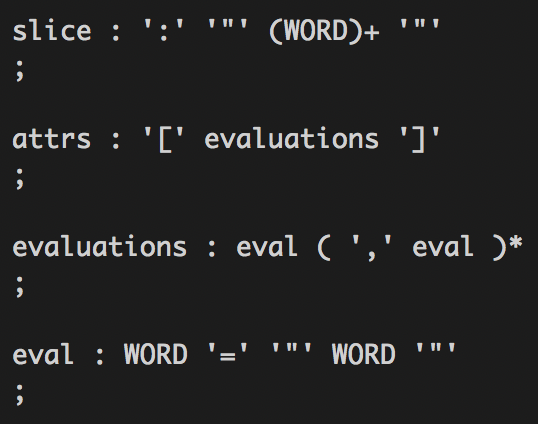
\includegraphics[width=8cm]{images/META_slice_attrs.png}
    \caption{DSL slice/attrs/evaluations/eval production.}
    \label{fig:dsl_slice_production}
\end{figure}

Inside the \textbf{slice} production, a list of words can be written. These are the words that will then be used to build the lexical part of the generated grammar. Also, when specifying attributes, the student must assign a value for each attribute that will then be used to validate each component of the sentence.

For a better understanding of the three main categories (structure, errors and input), bellow there is an example that is based on the first case study, and shows what the semantic of the teacher should look like.

% Exemplo de frase da meta gramática (parte do professor)
\begin{figure}[h]
    \centering
    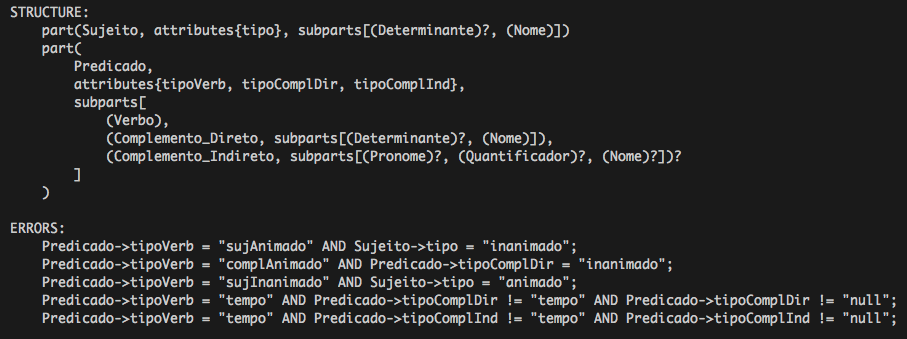
\includegraphics[width=15cm]{images/phrase_meta_grammar.png}
    \caption{Example of a possible sentence structure.}
    \label{fig:meta_grammar_teacher}
\end{figure}

In the case of the student, this is the semantic that should be used and one of the many examples that fit into the defined structured.

% Exemplo de frase da meta gramática (parte do aluno)
\begin{figure}[h]
    \centering
    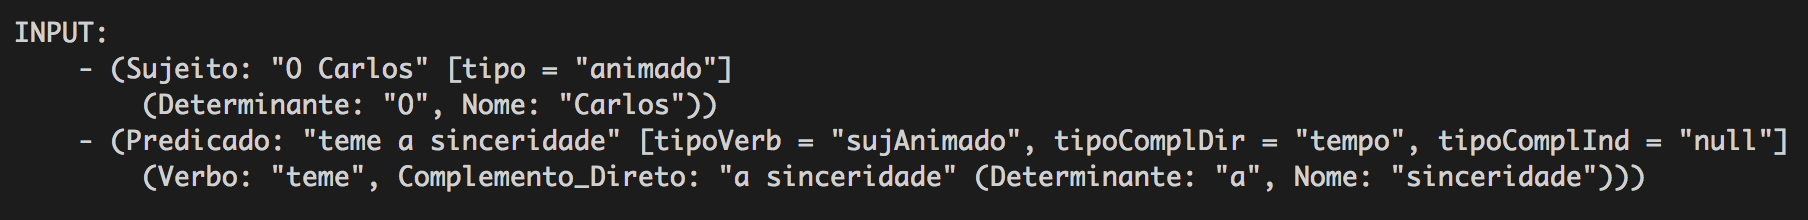
\includegraphics[width=15cm]{images/INPUT_meta_grammar_example.png}
    \caption{Example of the students parsing.}
    \label{fig:meta_grammar_student}
\end{figure}

\section{Case Study}
After the conception of a possible system architecture and DSL, the first task was to define the \textsc{DSL} that was supposed to be generated by the ``meta-language'' processor. This \textsc{DSL} would be the translation of the previously defined language into \textsc{ANTLR} instructions, that have as main purpose to verify the sentences written by the students. The \textsc{DSL} design consists in slicing the sentence into main parts, with each main part possibly having more parts into them. These parts are supposed to be specified by the teacher, but in this context, as a case study, it was assumed that a structure is predefined.

\subsection{Attribute Validation}
This case study intends to validate sentence components based on their attributes, where certain components require certain types of attributes in different components of the sentence. The example shows that one sentence is divided into two main parts: a subject (\underline{sujeito}) and a predicate (\underline{predicado}). The subject is then subdivided into a possible pronoun (\underline{pronome}) and a noun (\underline{nome}), which are then matched with a word (in this example the words are predefined). The predicate is composed by the verb (\underline{verbo}) and two complements that are directly and indirectly (\underline{complementoDireto} and \underline{complementoIndireto}) connected to the verb. Both these complements are composed by a possible pronoun or determinant (\underline{determinante}) followed by a quantifier (\underline{quantificador}) and a noun. The verb is, like the noun, predefined.

% Excerto da DSL para caso de estudo.
\begin{figure}[h]
    \centering
    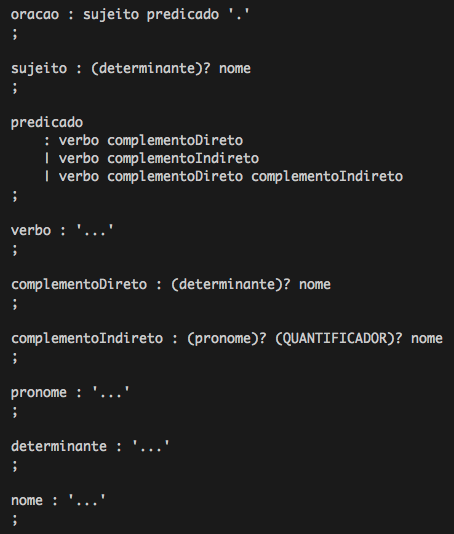
\includegraphics[width=12cm]{images/dsl_excerpt.png}
    \caption{Example DSL excerpt.}
    \label{fig:dsl_excerpt}
\end{figure}

All that is left to do, is to start evaluating all the different attributes that each component has, and to check if the sentence provided by the student is, according to the rules, valid. 

As shown in the excerpt below, and based on different set of attributes and rules, if the verb requires an \textbf{animated} subject then if the subject is \textbf{inanimated} an error message should appear, and notify the student of that same error. These error messages are the translation of the ``ERRORS'' block explained on the previous section.

% Excerto da validação de atributos na gramática.
\begin{figure}[h]
    \centering
    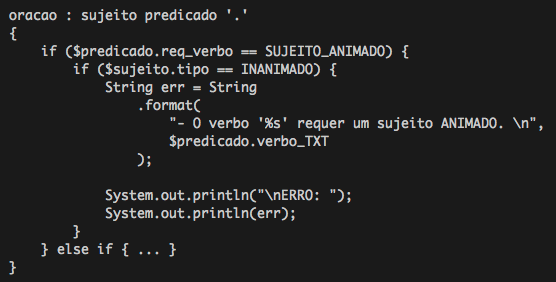
\includegraphics[width=12cm]{images/dsl_validation.png}
    \caption{Example DSL attribute validation.}
    \label{fig:dsl_attribute_validation}
\end{figure}

To conclude, if we use as an input a sentence like
\begin{description}
    O Carlos teme a sinceridade.
\end{description}
the sentence is accepted because, firstly, the structure is correct, and every component is in the right place, and secondly, all the attributes obey to the rules. As another example, if we use as an input other sentence for example \begin{description}
    O acidente teme a sinceridade.
\end{description}
we get an error which indicates that the verb ``teme" requires an animated subject, and ``acidente'' belongs to the subject that has an inanimated property.

% Exemplo de um erro na dsl de teste.
\begin{figure}[h]
    \centering
    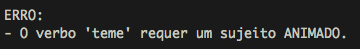
\includegraphics[width=10cm]{images/animated_subject_error.png}
    \caption{Example of an error message.}
    \label{fig:error_message_dsl}
\end{figure}

\subsection{Number and Gender}
This case study, based on the same \textsc{DSL} excerpt [\ref{fig:dsl_excerpt}], intends to validade the gender and number within the subject. Two of the productions, \textbf{determinante} and \textbf{nome}, need to be in concordance when it comes to gender and number. By using synthesized attributes, we can return the genders and numbers of the given words.

% produção do determinante dsl excerpt
\begin{figure}[h]
    \centering
    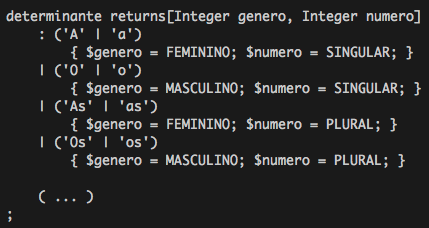
\includegraphics[width=10cm]{images/dsl_determinante_excerpt.png}
    \caption{Excerpt of the 'determinante' production.}
    \label{fig:determinante_dsl_excerpt}
\end{figure}

% produção do nome dsl excerpt
\begin{figure}[h]
    \centering
    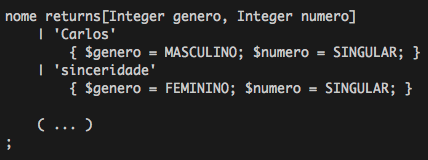
\includegraphics[width=10cm]{images/dsl_nome_excerpt.png}
    \caption{Excerpt of the 'nome' production.}
    \label{fig:nome_dsl_excerpt}
\end{figure}

Within the \textbf{sujeito} production, we can perform these two evaluations, and check if the sentence provided by the student is, again, according to the rules, valid.

% produção do sujeito dsl excerpt
\begin{figure}[h]
    \centering
    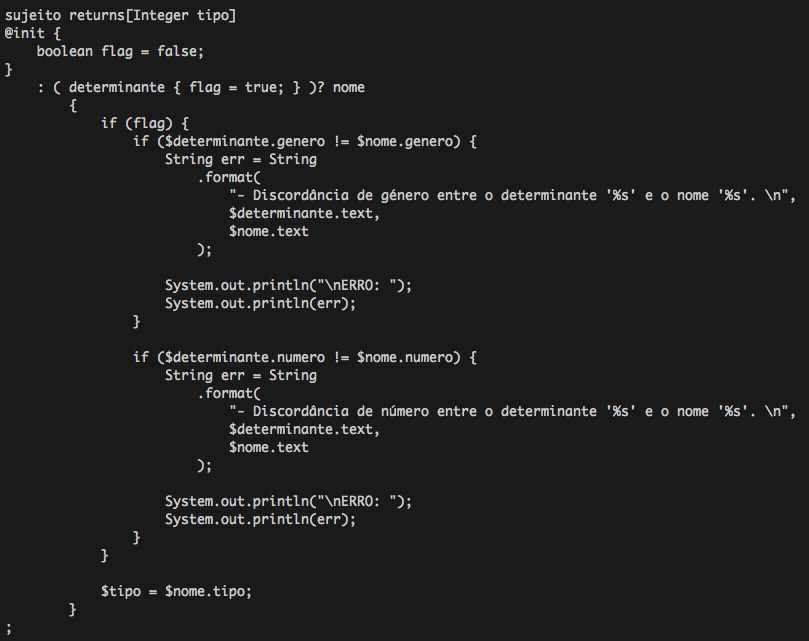
\includegraphics[width=13cm]{images/dsl_GenderNumber_validation.png}
    \caption{Example of gender/number validation within the 'sujeito' production.}
    \label{fig:sujeito_dsl_excerpt}
\end{figure}

To conclude this case study, if we use a similar input, but with an error
\begin{description}
    A Carlos teme a sinceridade.
\end{description}
we get a message indicating that the determinant and noun have a different gender.

% erro gender dsl excerpt
\begin{figure}[h]
    \centering
    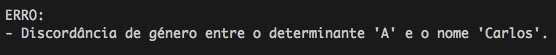
\includegraphics[width=11cm]{images/dsl_gender_error.png}
    \caption{Example of a gender error message.}
    \label{fig:erro_gender_dsl_excerpt}
\end{figure}

\noindent Using another input, for example
\begin{description}
    Os Carlos teme a sinceridade.
\end{description}
we can see that the gender matches, but the number in incorrect. Likewise, we get an error.

% erro number dsl excerpt
\begin{figure}[h]
    \centering
    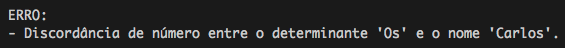
\includegraphics[width=11cm]{images/dsl_number_error.png}
    \caption{Example of a number error message.}
    \label{fig:erro_number_dsl_excerpt}
\end{figure}